\section{Revenue and Rewards}\label{sec:revenue}

\subsubsection*{What is colony revenue?}
A colony may sell goods and services in exchange for tokens, for Ether or for one of the  ERC20 tokens whitelisted for use on the network. Whenever a colony receives such payments, we say that the colony has earned \emph{revenue}.\footnote{A colony contract can of course receive any tokens, even those that are not whitelisted. Only payments that can be used within a colony for funding proposals and tasks payouts count as revenue.}

Revenue is distinct from a colony's working capital. The latter is the sum of all tokens held by the colony for use in funding requests i.e. the funds in the funding pot belonging to the root domain in the colony (see Section \ref{sec:finance}), while the former, revenue, is implicitly defined as the colony's token holdings not accounted for in any of the existing pots.

\subsubsection*{What are colony rewards?}
There is some expectation that some fraction of any Ether or other valuable tokens earned by the colony are paid out to their token holding members. `Members', in this context, means accounts holding both tokens and reputation in the colony. Whenever a colony distributes a portion of earned revenue to its token holding members, we say that the colony is paying out \emph{rewards}. It is expected that most of the revenue will \emph{not} go towards rewards, but towards replenishing the working capital.

\subsection{Processing revenue}
Revenue accumulates as the colony receives transfers of tokens. In order to be processed, a user has to make a special `claim revenue' transaction, indicating for which token they wish to process accumulated revenue.

The transaction then calculates the amount of token-denominated revenue that has accumulated since the last such transaction, and transfers some (small) percentage to the colony rewards pot. The remainder is then made available to the colony as working capital. The percentage split can be changed by the colony based on a colony-wide vote of tokens and reputation, requiring a majority of both tokens and reputation.

\subsection{Claiming rewards from the rewards pot}\label{sec:claimrewards}
Rewards accumulate in the rewards pot. To trigger an actual payout to users (i.e. to make rewards claimable) a special type of proposal is made, proposing that all users should receive a payout based on the reward pot's holdings.

This reward payout proposal includes the specific currency that should be paid, and only one currency is handled at a time. In the event that the proposal is approved by vote of reputation, then all user's tokens are locked until they claim their payout. Locking is necessary, because the token balance of each account factors into the rewards formula of equation \eqref{eq:reward-claim}. Locking is triggered by incrementing the colony's `most recent payout' counter.

Our currency contract contains a locking mechanism ensuring that a user cannot move tokens while they have (token-weighted) votes to reveal; we use the same mechanism here to ensure that a user cannot move tokens after a payout is approved by the members of the colony but before the user has claimed their rewards. The colony has a counter for each user that is incremented whenever they claim a payout; they can also waive their claim to a payout that will increment this counter.

While it is of course up to the members of each individual colony to decide, it is advisable that these payout proposals should only be accepted sporadically to keep the gas costs low for the users claiming their payouts, as well as simply to not be a nuisance to the users continually finding their tokens locked.

\textbf{Rewards are only available to accounts that hold both tokens and reputation}, and the amount claimable by each account depends on \emph{both} token balance and reputation (see equation \eqref{eq:reward-claim} below). Therefore we need to have a similar behaviour to `lock' the reputation of the users for the payout. When a payout is activated, the current state of the reputation tree is recorded in the payout itself. Users are paid out according to their reputation in this state, rather than the most recent state, to ensure all users get an appropriate payout and to avoid exploiting the system (which might otherwise be possible via e.g. delaying reward collection until after completing a task, increasing their reputation).

\subsubsection*{The rewards formula}
The amount that each user ($u_i$) of a colony ($\mathcal{C}$) is entitled to claim ($p_i$) is a function of their colony token holdings ($t_i$) and their total reputation in the colony ($r_i$):

\begin{equation}\label{eq:reward-claim}
 p_i = \left(\frac{t_i r_i}{T \times R}\right)^{\frac{1}{2}} \qquad \textnormal{where} \quad T = \sum\limits_{u_j\in \mathcal{C}} t_j \quad\textnormal{and}\quad R = \sum\limits_{u_j\in \mathcal{C}} r_j.
\end{equation}

This is a (normalised) geometric average of the user's token holdings and reputation. We note that this is very unlikely to payout all the tokens set aside for a payout --- the only way it would do so is if everyone had the same proportion of reputation in the colony as they did proportion of tokens in the colony. However, the geometric average is the natural way to fairly capture the influence of two variables with different ranges, and ensures that large token holders must earn large amounts of reputation to get the most from the payouts. The total reputation and user reputation in the colony are all provable on-chain at claim time via a Merkle proof that the \ascode{ReputationRootHash} (Section \ref{sec:reputationmining}) contains some values claimed by the user; the user's balance of colony tokens and the total number of tokens issued is trivial to lookup.

After some sufficiently long period of time (\rewardclaimduration\ days), all unclaimed tokens can be reclaimed on behalf of the colony by a user, and the payout closed. Any users that have not claimed their payout by that point will still have their tokens locked, and they will remain locked until they issue a transaction waiving their claim to the payout (indeed, they already passively did this by not claiming it in a timely fashion). Unclaimed tokens are returned to the rewards pot and become part of the next reward cycle.

\subsection{The revenue model of the Colony Network}\label{sec:networkrevenue}
The Colony Network must be able to sustain itself. In particular, the \rc\ (which ultimately is in control of the Colony Network) maintains the contracts that underpin the network and develops new functionality for the network, the development of which needs to be paid for. Long term, the development and maintenance of the network (including the reputation system) needs to be financed by the network itself.

\subsubsection{The network fee}\label{sec:networkfee}
We propose a fee that is levied on task payments made. When a user claims payment for a task they have done, and the funds leave the control of the Colony, some small fraction is paid to the network. A cartoon showing the revenue split is show in Figure \ref{fig:revenueSplit}.

\begin{figure}[htp]
\centering
 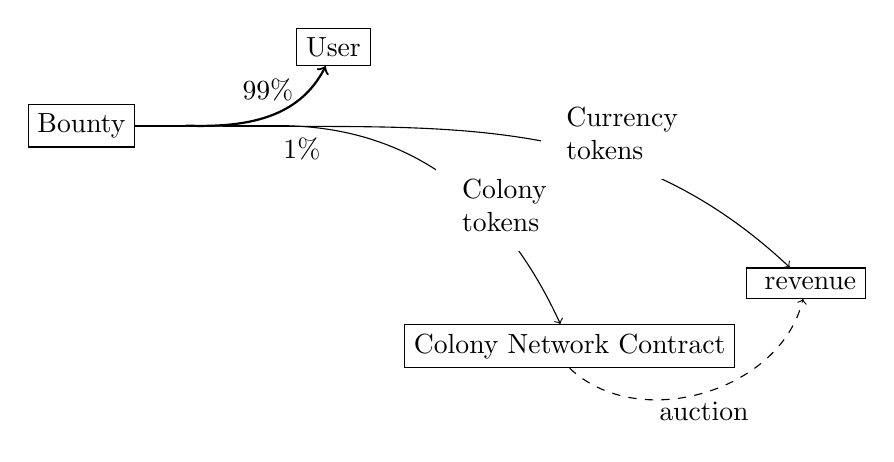
\begin{tikzpicture}
  \node at (-4,0) (dummy) {};
  \node[draw] at (-5.2,0) (bountybox) {Bounty};
  \node at (-2.8,0) (bounty) {}
   (bountybox.east) edge[-, thick] (dummy.east)
   (dummy.east) edge[-] (bounty.east);
   \node at (-2.4,-0.3) {{1\%}};
  \node[draw] at (-2,1) (user) {User};
  \node[draw] at (1,-2.8) (cnc) {Colony Network Contract};
  \node[draw] at (4,-2) (root) {\rc\ revenue}
    (dummy.east) edge[->, bend right=40,out=-25,thick] node[above=2pt] {99{\%}} (user)
    (dummy.east) edge[->, bend left=30,out=12] node[fill=white,right=10pt] {\begin{tabular}{l} Currency \\ tokens\end{tabular}} (root)
    (bounty.east) edge[->, bend left=30,out=35] node[fill=white, below right=-5pt] {\begin{tabular}{l} Colony \\ tokens\end{tabular}} (cnc)
    (cnc.south) edge[->, bend right=60, dashed] node[below] {auction} (root)
    ;
 \end{tikzpicture}
 \caption{Summary of the revenue split upon payout for a task.}
 \label{fig:revenueSplit}

\end{figure}

The fees thus collected are sent to either the \rc\ (if the payment was in Ether or another whitelisted token) or the Colony Network Contract (if it was in a colony's token).

This idea of a fee is a little unusual for such a decentralised system. One of the appeals of decentralised systems on Ethereum is that other than gas costs, they do not seek rent and are free to use. However, the Network Fee is vital in ensuring the game theoretic security of the Colony Network's reputation mining and governance processes by providing underlying value to the CLNY held by Meta Colony members. Importantly, this fee is not payable to any centrally controlled entity, but rather to the Meta Colony. Anybody may contribute to the Meta Colony and claim a share of these fees proportional to their contribution. We believe that the benefit of being part of a secure, well supported network will ultimately be appealing enough that a small fee to pay for its existence will be acceptable.

The presence of this fee means we have to make some considerations which would otherwise be irrelevant. Primarily, we will need to make `piggyback' contracts as hard as possible to make that might e.g. be used to pay out a task reward when a task was completed, but without sending the fee.

\subsubsection{The token auction}
As the network fee may be denominated in any ERC20 token, there is a need for a mechanism to liquidate arbitrary bundles of tokens -- the token auction. The colony tokens collected are auctioned off by the Colony Network Contract, with the auctions denominated in \rcts, the proceeds of which are burnt. These auctions --- one for each type of token collected --- occur on a regular basis of once a month.

We believe such a mechanism will be beneficial for the \rcths\ (whose \rcts\ gain value by having an explicit use beyond reputation mining) and the \rc\ itself (by reducing the supply of \rcts\ and thus making any future minting more valuable). It also provides an immediate mechanism of price discovery for the colony tokens, which are unlikely to be traded on third-party exchanges until much later in the lifetime of the colony. By auctioning off the collected tokens, we also prevent the \rc\ collecting a large number of different tokens that it has to manage, which would prove cumbersome and annoying for the colony.



